\chapter{Preface}

This manual is for newcomers to Mimetic Operator's Library
Enhanced~\cite{Corbino2024} (MOLE) with a foundation in Numerical
Analysis for Partial Differential Equations (PDEs).
The library is growing with examples implemented with sparse matrix
data structures in
\href{https://octave.org}{GNU Octave}/
\href{https://www.mathworks.com/products/matlab.html}{MATLAB},
and \href{https://isocpp.org}{C++}.
In addition, most of these examples are provided using a
\href{https://www.python.org}{Python} module called
\texttt{pyMOLE}~\cite{Aznarán2025}.
Therefore, understanding this implementation of mimetic operators
will allow users to translate the algorithms into other
high-performance scientific programming languages such as
\href{https://julialang.org}{Julia},
\href{https://fortran-lang.org}{Fortran},
\href{https://www.rust-lang.org}{Rust} and
\href{https://www.open-std.org/jtc1/sc22/wg14}{C}.

The main goal of this document is to provide clear and complete
explanations of these examples to help users understand the core
concepts and applications of the library.
We would like to thank Professor
\href{https://ctivitae.concytec.gob.pe/appDirectorioCTI/VerDatosInvestigador.do?id_investigador=45848}{Miguel Dumett}
of the Computational Science Research Center at San Diego State
University and the National University of Trujillo for organizing
MOLE courses.

\begin{figure}[ht!]
	\centering
	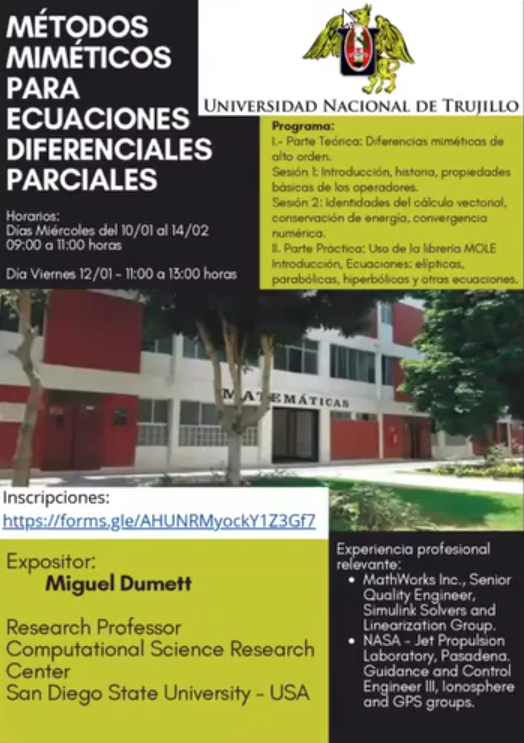
\includegraphics[width=.32\paperwidth]{mole2024}\quad
	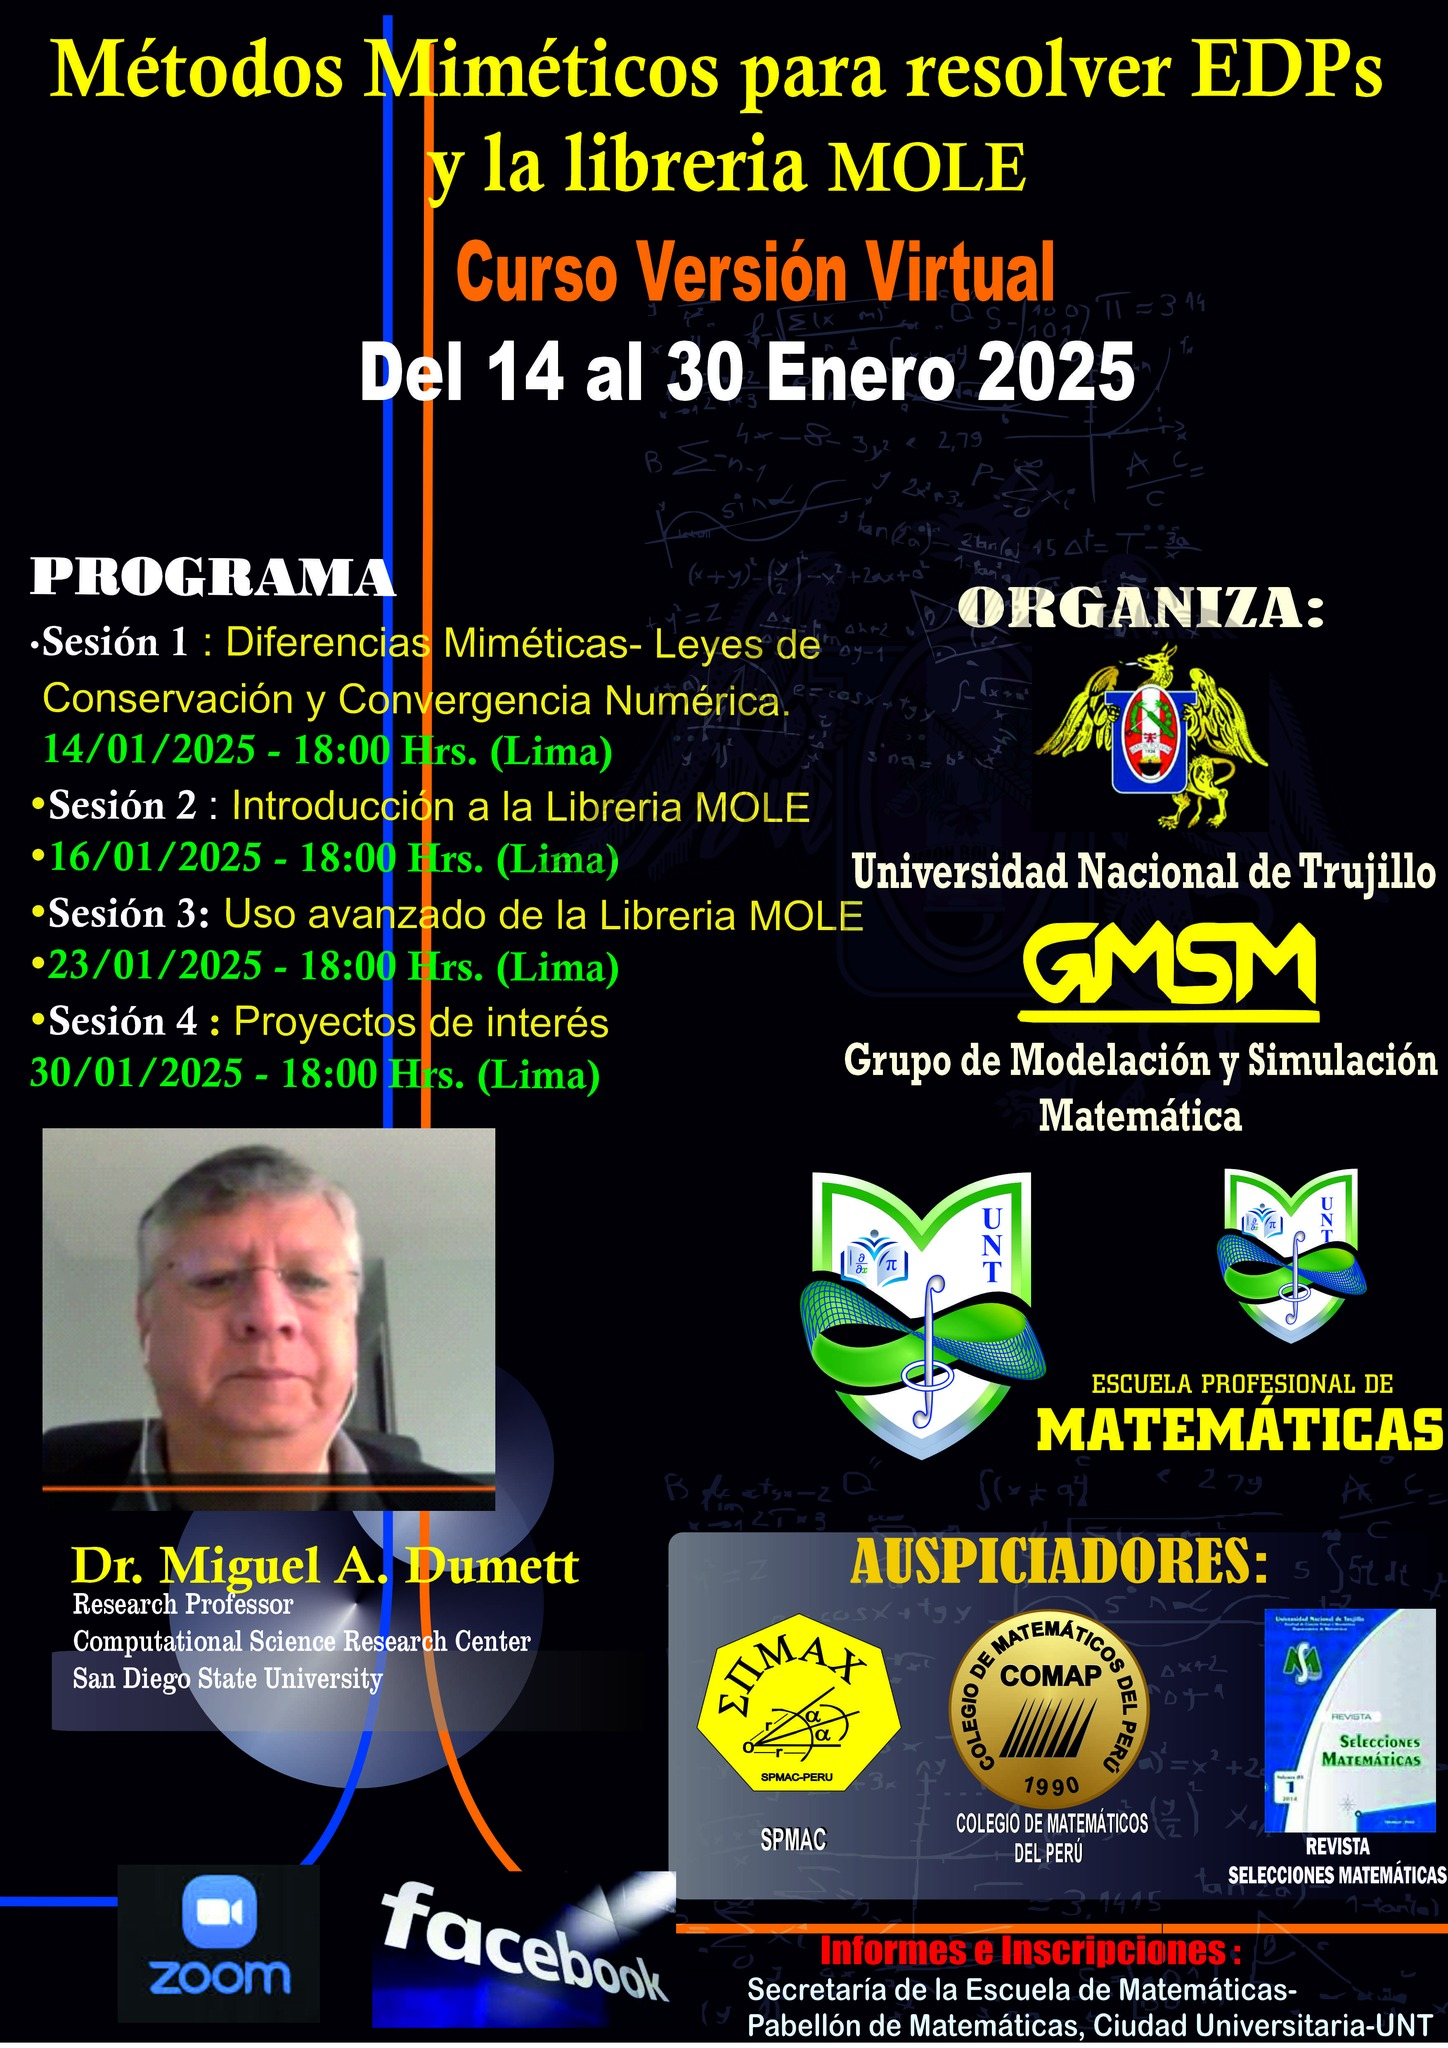
\includegraphics[width=.32\paperwidth]{mole2025}
	\caption*{\bfseries Mimetic Methods courses in January and February 2024 and 2025.}
\end{figure}

\begin{flushright}
	Lima, Puno \hfill Carlos Aznarán \\[.5\baselineskip]

	April 2025 \hfill Adelaida Otazu
\end{flushright}
